\documentclass[tikz]{standalone}
\usepackage{mathtools}
\usetikzlibrary{angles, quotes}

\begin{document}
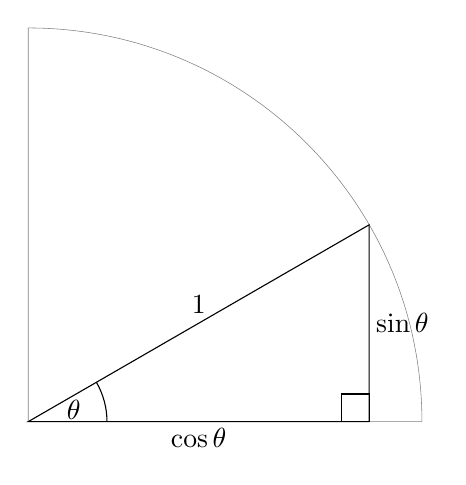
\begin{tikzpicture}[scale=5]
  \coordinate (A) at (0, 0);
  \coordinate (B) at (30:1);
  \coordinate (C) at (B |- {(1, 0)});

  \draw[help lines] (0, 1) -- (0, 0) --
    (1, 0) arc[start angle=0, end angle=90, radius=1] -- cycle;

  \draw (A) -- node[above] {$1$}
    (B) -- node[xshift=-1pt, right] {$\sin\theta$}
    (C) -- node[yshift=1pt, below] {$\cos\theta$} cycle;

  \draw pic[angle radius=10mm, draw=black, "$\theta$"] {angle=C--A--B};
  \draw (C) rectangle +(-2pt, 2pt);
\end{tikzpicture}
\end{document}

%%% Local Variables:
%%% mode: latex
%%% TeX-master: t
%%% End:
